\documentclass[11pt]{article}
\usepackage[left=20mm, right=20mm,top=20mm, bottom= 20mm]{geometry}
\usepackage{verbatim, graphicx, tcolorbox}
\usepackage{multirow, makecell, url}
\usepackage{subcaption}

\title{Factor Analysis Report for "Sleep Health and Lifestyle" Dataset}
\author{S/18/827 - J Kumudumali Sandaleka}
\date{\today}


\begin{document}
	
	\maketitle
	\setlength{\parindent}{0pt}
	\setlength{\parskip}{6pt}
	
	\section{Introduction}
		 Factor analysis (FA) is a fundamental statistical technique used for modelling observed variables and their covariance structure in terms of a smaller number of underlying unobservable (latent) "factors". These factors aim to explain the underlying structure or patterns within a dataset by identifying common variance among observed variables. \par 
		 
		 In this study, the "Sleep Health and Lifestyle" dataset is used to conduct factor analysis. This dataset comprises various variables related to sleeping and lifestyle. By applying factor analysis, my objective is to reduce the dimensionality of the dataset while retaining meaningful information. This process facilitates the interpretation and the understanding of the underlying factors influencing sleep and lifestyle.
		 
	\section{Methodology}
	The methodology section encompasses rigorous data preprocessing, exploratory factor analysis (EFA), and confirmatory factor analysis (CFA), ensuring a comprehensive understanding of latent factors and their relationships within the "Sleep Health and Lifestyle" dataset.
	
		\subsection{Dataset Description}
		The "Sleep Health and Lifestyle" dataset consists of 400 row and 13 columns, covering a range of variables including,
		
		\begin{enumerate}
			\item Person ID: An identifier for each individual.
			\item Gender: The gender of the person (Male/Female).
			\item Age: The age of the person in years.
			\item Occupation: The occupation or profession of the person.
			\item Sleep Duration (hours): The number of hours the person sleeps per day.
			\item Quality of Sleep (scale: 1-10): A subjective rating of the quality of sleep.
			\item Physical Activity Level (minutes/day): The number of minutes the person engages in physical activity daily.
			\item Stress Level (scale: 1-10): A subjective rating of the stress level experienced by the person, ranging from 1 to 10.
			\item BMI Category: The BMI category of the person (e.g., Underweight, Normal, Overweight).
			\item Blood Pressure (systolic/diastolic): The blood pressure measurement of the person.
			\item Heart Rate (bpm): The resting heart rate of the person in beats per minute.
			\item Daily Steps: The number of steps the person takes per day.
			\item Sleep Disorder: The presence or absence of a sleep disorder in the person (None, Insomnia, Sleep Apnea).
		\end{enumerate}
		
		\subsection{Factor Analysis}
			\subsubsection{Data Preprocessing}
			Before conducting factor analysis, the dataset was thoroughly preprocessed to ensure its integrity and suitability. This required addressing duplicate entries and missing values in addition to standardizing the data to reduce inconsistencies caused by disparate units of measurement.In this stage I observed that there are no outliers in this dataset.
		
			\subsubsection{Exploratory Factor Analysis (EFA)}
		 	The preliminary stage of the analysis focused on determining the optimal number of factors to extract from the dataset. Various techniques were employed for this purpose, including Jolliffe's Method and the scree plot, which aimed to identify factors explaining 80\% of the variance. EFA began with an initial factor analysis using Principal Component Analysis (PCA) or Maximum Likelihood Estimation (MLE) to establish loadings for each selected factor. To enhance interpretability, rotation techniques were applied.Finally, factor loading, commonalities, and uniqueness were interpreted for more understanding.
		 
			\subsubsection{Confirmatory Factor Analysis (CFA)}
			Following the exploratory phase, CFA was used to determine how well the hypothesized model fit the observed data. This involved defining the correlations between the factors and the observed variables and evaluating the fit of the model using a variety of fit indices, such as the Tucker-Lewis Index (TLI), Comparative Fit Index (CFI), Root Mean Square Error of Approximation (RMSEA), and chi-square test. These indices validate the underlying factor structure by showing how well the suggested model fits the observed data.
		
		In conclusion, the methodology included comprehensive data preprocessing, suitability assessment, exploratory factor analysis for factor extraction, and confirmatory factor analysis to validate the proposed model. These steps contribute to a thorough understanding of the dataset's latent factors and their relationships with observed variables.
		
	\newpage
	\section{Results and Discussion}
	
	In this section, we present the results of our analysis, beginning with an exploration of the basic assumptions underlying the factor analysis. We conducted Exploratory Factor Analysis (EFA) to identify underlying latent factors within the dataset, employing varimax rotation to enhance interpretability. The results of EFA provided insights into the structure of the data and potential underlying constructs. Following EFA, Confirmatory Factor Analysis (CFA) was performed to validate the factor structure identified in EFA.
	
		\subsection{Checking the basic assumptions}
			\subsubsection{Sampling adequacy}
			The Kaiser-Meyer-Olkin (KMO) measure of sampling adequacy is a better measure of factor-ability. The minimum acceptable value is 0.50. \par
			
			\begin{tcolorbox}[colback=white,colframe=black]
				\begin{verbatim}
					Kaiser-Meyer-Olkin factor adequacy
					Call: KMO(r = standardized_data)
					Overall MSA =  0.76
					MSA for each item = 
					age         sleep_duration    quality_of_sleep     stress_level     bmi_category 
					0.77             0.85             0.71             0.73             0.83 
					systolic_bp      diastolic_bp    heart_rate        sleep_disorder 
					0.71             0.72             0.81             0.79 
				\end{verbatim}
			\end{tcolorbox}
			
			Initially, the KMO analysis for the "Sleep Health and Lifestyle" dataset yielded an overall Measure of Sampling Adequacy (MSA) of 0.59, which suggests marginal adequacy. After removing the variables with low MSA values, a second KMO analysis was conducted, resulting in a substantially improved overall MSA of 0.76. This indicates a higher level of sampling adequacy, suggesting that the remaining variables are more suitable for factor analysis.
			
			\subsubsection{Significance of the multiple correlations}
			This evaluates whether or not the variables intercorrelate at all, by evaluating the observed correlation matrix against an “identity matrix”.
			
			\begin{tcolorbox}[colback=white,colframe=black]
				\begin{verbatim}
					R was not square, finding R from data
					$chisq             $p.value	        $df
					[1] 3709.504          0              36
				\end{verbatim}
			\end{tcolorbox}
			
			
			The p-value of 0 indicates that the observed correlation matrix significantly differs from an identity matrix, as it is less than the conventional significance level of 0.05. Therefore, we reject the null hypothesis, suggesting that there are correlations among the variables in the dataset.
		\newpage
		\subsection{Explanatory Factor Analysis (EFA)}
		 The Explanatory Factor Analysis (EFA) section delves into determining the appropriate number of factors to extract and estimating factor model parameters, revealing insights into underlying constructs within the dataset.
			\subsubsection{Determining the Number of Factors to Extract}
			After checking basic assumptions, we need to clarify that how many components or factors that we are going to extract. For this purposes, we can use some methods or criterion:
		
			\begin{enumerate}
				\item \textbf{Eigenvalues / Variances} 
				\begin{table}[h]
					\centering
					\resizebox{12cm}{!}{%
						\begin{tabular}{|c|c|c|c|}
							\hline
							\textbf{Factor} & \textbf{Eigen value} & \textbf{Proportion due to factor} & \textbf{Cumulative Proportion (\%)} \\ \hline
							1               & 4.0555               & 0.4506                            & 45.06                               \\ \hline
							2               & 3.0713               & 0.3413                            & 79.19                               \\ \hline
							3               & 0.6944               & 0.0772                            & 86.91                               \\ \hline
							4               & 0.4476               & 0.0497                            & 91.88                               \\ \hline
							5               & 0.2858               & 0.0318                            & 95.06                               \\ \hline
							6               & 0.2507               & 0.0279                            & 97.85                               \\ \hline
							7               & 0.1176               & 0.0131                            & 99.16                               \\ \hline
							8               & 0.0511               & 0.0057                            & 99.73                               \\ \hline
							9               & 0.0206                     & 0.0029                            & 100.02                              \\ \hline
						\end{tabular}%
					}
					%\caption{Eigen Values \& Variance }
					\label{tab:eigen_val}
				\end{table}
				
				Based on the Jolliffe`s method, it appears that the first two factors contribute significantly to the variance, with eigenvalues above 0.7. First three factors explains approximately 86.91\% of the total variance, suggesting that they capture a substantial portion of the variability in the dataset.
				
				\item \textbf{Scree Plot}
				\begin{figure}[h]
					\centering
					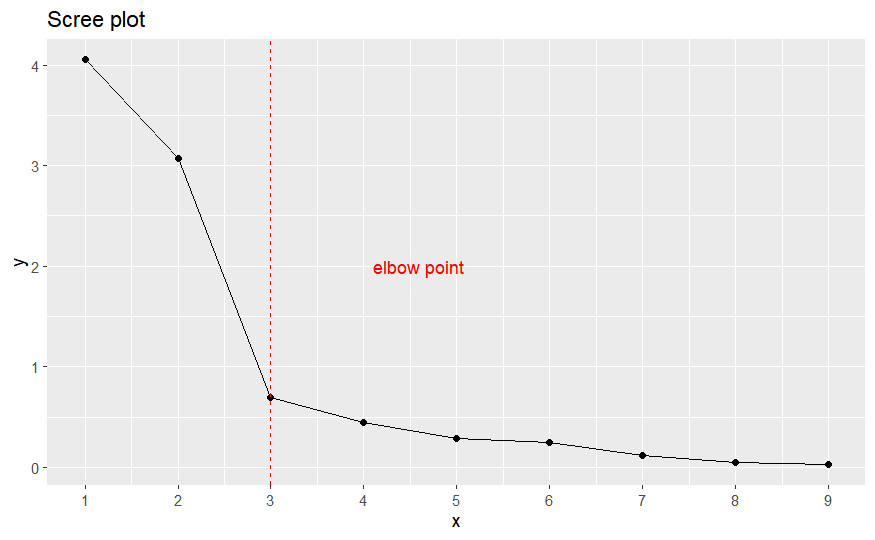
\includegraphics[width=10cm]{Images/scree_plot}
					\label{fig:screeplot}
				\end{figure}
				
				The scree plot shows the eigenvalues plotted against the factor number. The first three factors lie on the elbow. 
			\end{enumerate}
			
			Considering the findings of the scree plot and eigen values - variance we are positive that extracting three factors for our factor analysis of the "Sleep Health and Lifestyle" dataset is appropriate and meaningful.
			
			\subsubsection{Estimate the factor model parameters}
			In exploratory factor analysis (EFA), begin by conducting an initial factor analysis to determine the loadings for each selected factor. Two commonly used methods are Principal Component Analysis (PCA) and Maximum Likelihood Estimation (MLE):
			
	
			\begin{table}[h]
				\centering
				\resizebox{11cm}{!}{%
					\begin{tabular}{l|rrr|r|rrr|}
						\cline{2-4} \cline{6-8}
						& \multicolumn{3}{c|}{\textbf{PCA Method}}                                                                  & \multicolumn{1}{l|}{} & \multicolumn{3}{l|}{\textbf{MLE Method}}                                                                  \\ \cline{1-4} \cline{6-8} 
						\multicolumn{1}{|c|}{\textbf{Variable}} & \multicolumn{1}{c|}{\textbf{PC1}} & \multicolumn{1}{c|}{\textbf{PC2}} & \multicolumn{1}{c|}{\textbf{PC3}} & \multicolumn{1}{l|}{} & \multicolumn{1}{l|}{\textbf{ML1}} & \multicolumn{1}{l|}{\textbf{ML2}} & \multicolumn{1}{l|}{\textbf{ML3}} \\ \cline{1-4} \cline{6-8} 
						\multicolumn{1}{|l|}{Age}               & \multicolumn{1}{r|}{0.5}          & \multicolumn{1}{r|}{0.65}         & 0.17                              &                       & \multicolumn{1}{r|}{0.65}         & \multicolumn{1}{r|}{0.51}         & 0.17                              \\ \cline{1-4} \cline{6-8} 
						\multicolumn{1}{|l|}{Sleep Duration}    & \multicolumn{1}{r|}{0.83}         & \multicolumn{1}{r|}{-0.03}        & -0.29                             &                       & \multicolumn{1}{r|}{-0.03}        & \multicolumn{1}{r|}{0.85}         & -0.28                             \\ \cline{1-4} \cline{6-8} 
						\multicolumn{1}{|l|}{Quality of Sleep}  & \multicolumn{1}{r|}{0.97}         & \multicolumn{1}{r|}{0.03}         & -0.25                             &                       & \multicolumn{1}{r|}{0.04}         & \multicolumn{1}{r|}{0.97}         & -0.25                             \\ \cline{1-4} \cline{6-8} 
						\multicolumn{1}{|l|}{Stress Level}      & \multicolumn{1}{r|}{-0.94}        & \multicolumn{1}{r|}{0.01}         & -0.01                             &                       & \multicolumn{1}{r|}{0}            & \multicolumn{1}{r|}{-0.93}        & 0.01                              \\ \cline{1-4} \cline{6-8} 
						\multicolumn{1}{|l|}{BMI Category}      & \multicolumn{1}{r|}{-0.21}        & \multicolumn{1}{r|}{0.66}         & 0.45                              &                       & \multicolumn{1}{r|}{0.62}         & \multicolumn{1}{r|}{-0.19}        & 0.5                               \\ \cline{1-4} \cline{6-8} 
						\multicolumn{1}{|l|}{Systolic BP}       & \multicolumn{1}{r|}{-0.11}        & \multicolumn{1}{r|}{0.98}         & 0.15                              &                       & \multicolumn{1}{r|}{0.97}         & \multicolumn{1}{r|}{-0.11}        & 0.19                              \\ \cline{1-4} \cline{6-8} 
						\multicolumn{1}{|l|}{Diastolic BP}      & \multicolumn{1}{r|}{-0.1}         & \multicolumn{1}{r|}{0.95}         & 0.15                              &                       & \multicolumn{1}{r|}{0.95}         & \multicolumn{1}{r|}{-0.1}         & 0.19                              \\ \cline{1-4} \cline{6-8} 
						\multicolumn{1}{|l|}{Heart Rate}        & \multicolumn{1}{r|}{-0.69}        & \multicolumn{1}{r|}{0.23}         & 0.01                              &                       & \multicolumn{1}{r|}{0.22}         & \multicolumn{1}{r|}{-0.69}        & 0.02                              \\ \cline{1-4} \cline{6-8} 
						\multicolumn{1}{|l|}{Sleep Disorder}    & \multicolumn{1}{r|}{-0.19}        & \multicolumn{1}{r|}{0.41}         & 0.74                              &                       & \multicolumn{1}{r|}{0.38}         & \multicolumn{1}{r|}{-0.19}        & 0.77                              \\ \cline{1-4} \cline{6-8} 
					\end{tabular}%
				}
				%\caption{}
				\label{tab:pca_mle}
			\end{table}
			
		In this analysis, both PCA and ML methods revealed that all three factors extracted from the analysis are statistically significant. The three factors together explain around 80\% of the total variance in the data and factor loadings are also closer to -1 or +1, indicating stronger relationships between variables and factors in both methods. In terms of correlation patterns, PCA identifies factor 3 solely correlated with sleeping disorder, whereas ML shows factor 3 correlated with both sleeping disorder and BMI category.
			
		Consequently, the Maximum Likelihood method is chosen for further analysis due to its more reliable factor loadings and better representation of the relationships between variables and factors.
	
	
		\subsubsection{Factor Rotations}
			
		Factor extraction aims to identify underlying constructs in the data, but these factors can be challenging to interpret directly. To address this issue, rotation techniques are used. 		
			
	
		\begin{table}[h]
			\centering
			\resizebox{10cm}{!}{%
				\begin{tabular}{c|ccc|c|ccc|}
					\cline{2-4} \cline{6-8}
					& \multicolumn{3}{c|}{\textbf{\begin{tabular}[c]{@{}c@{}}Unrotated \\ Factor Loadings\end{tabular}}} &  & \multicolumn{3}{c|}{\textbf{\begin{tabular}[c]{@{}c@{}}Rotated Factor\\ Loadings\end{tabular}}} \\ \cline{1-4} \cline{6-8} 
					\multicolumn{1}{|c|}{\textbf{Variable}} & \multicolumn{1}{c|}{\textbf{F1}}       & \multicolumn{1}{c|}{\textbf{F2}}       & \textbf{F3}      &  & \multicolumn{1}{c|}{\textbf{F1}}      & \multicolumn{1}{c|}{\textbf{F2}}      & \textbf{F3}     \\ \cline{1-4} \cline{6-8} 
					\multicolumn{1}{|c|}{Age}               & \multicolumn{1}{c|}{0.18}              & \multicolumn{1}{c|}{\textbf{0.8}}      & 0.18             &  & \multicolumn{1}{c|}{\textbf{0.65}}    & \multicolumn{1}{c|}{\textbf{0.51}}    & 0.17            \\ \cline{1-4} \cline{6-8} 
					\multicolumn{1}{|c|}{Sleep Duration}    & \multicolumn{1}{c|}{\textbf{-0.65}}    & \multicolumn{1}{c|}{\textbf{0.6}}      & -0.05            &  & \multicolumn{1}{c|}{-0.03}            & \multicolumn{1}{c|}{\textbf{0.85}}    & -0.28           \\ \cline{1-4} \cline{6-8} 
					\multicolumn{1}{|c|}{Quality of Sleep}  & \multicolumn{1}{c|}{\textbf{-0.67}}    & \multicolumn{1}{c|}{\textbf{0.74}}     & 0                &  & \multicolumn{1}{c|}{0.04}             & \multicolumn{1}{c|}{\textbf{0.97}}    & -0.25           \\ \cline{1-4} \cline{6-8} 
					\multicolumn{1}{|c|}{Stress Level}      & \multicolumn{1}{c|}{\textbf{0.6}}      & \multicolumn{1}{c|}{\textbf{-0.67}}    & -0.22            &  & \multicolumn{1}{c|}{0}                & \multicolumn{1}{c|}{\textbf{-0.93}}   & 0.01            \\ \cline{1-4} \cline{6-8} 
					\multicolumn{1}{|c|}{BMI Category}      & \multicolumn{1}{c|}{\textbf{0.71}}     & \multicolumn{1}{c|}{0.26}              & 0.33             &  & \multicolumn{1}{c|}{\textbf{0.62}}    & \multicolumn{1}{c|}{-0.19}            & \textbf{0.5}    \\ \cline{1-4} \cline{6-8} 
					\multicolumn{1}{|c|}{Systolic BP}       & \multicolumn{1}{c|}{\textbf{0.81}}     & \multicolumn{1}{c|}{\textbf{0.58}}     & -0.01            &  & \multicolumn{1}{c|}{\textbf{0.97}}    & \multicolumn{1}{c|}{-0.11}            & 0.19            \\ \cline{1-4} \cline{6-8} 
					\multicolumn{1}{|c|}{Diastolic BP}      & \multicolumn{1}{c|}{\textbf{0.79}}     & \multicolumn{1}{c|}{\textbf{0.57}}     & -0.01            &  & \multicolumn{1}{c|}{\textbf{0.95}}    & \multicolumn{1}{c|}{-0.1}             & 0.19            \\ \cline{1-4} \cline{6-8} 
					\multicolumn{1}{|c|}{Heart Rate}        & \multicolumn{1}{c|}{\textbf{0.6}}      & \multicolumn{1}{c|}{-0.35}             & -0.19            &  & \multicolumn{1}{c|}{0.22}             & \multicolumn{1}{c|}{\textbf{-0.69}}   & 0.02            \\ \cline{1-4} \cline{6-8} 
					\multicolumn{1}{|c|}{Sleep Disorder}    & \multicolumn{1}{c|}{\textbf{0.61}}     & \multicolumn{1}{c|}{0.08}              & \textbf{0.62}    &  & \multicolumn{1}{c|}{0.38}             & \multicolumn{1}{c|}{-0.19}            & \textbf{0.77}   \\ \cline{1-4} \cline{6-8} 
					\hline
				\end{tabular}%
			}
			%\caption{}
			\label{tab:rotated_unrotated}
		\end{table}
					
		According to the results, the rotated factor loadings demonstrate notable correlations closer to 1 and -1, indicating stronger and more meaningful relationships between variables and factors. Given these findings, it is sound to continue with factors rotated using varimax rotation. 
			
		\newpage
		\subsubsection{Varimax - MLE Factor Model}
		
		\begin{table}[h]
			\centering
			\resizebox{12cm}{!}{%
				\begin{tabular}{|c|ccc|cc}
					\hline
					\multirow{2}{*}{\textbf{Variable}}                                       & \multicolumn{3}{c|}{\textbf{\begin{tabular}[c]{@{}c@{}}Estimated Factor \\ Loadings\end{tabular}}} & \multicolumn{1}{c|}{\textbf{Communalities}} & \multicolumn{1}{c|}{\textbf{Specific Variances}} \\ \cline{2-6} 
					& \multicolumn{1}{c|}{\textbf{F1}}       & \multicolumn{1}{c|}{\textbf{F2}}       & \textbf{F3}      & \multicolumn{1}{c|}{\textbf{$h^2_i$}}       & \multicolumn{1}{c|}{\textbf{$\psi = 1 - h^2$}}   \\ \hline
					Age                                                                      & \multicolumn{1}{c|}{\textbf{0.65}}     & \multicolumn{1}{c|}{\textbf{0.51}}     & 0.17             & \multicolumn{1}{c|}{0.7084155}              & \multicolumn{1}{c|}{0.291584545}                 \\ \hline
					Sleep Duration                                                           & \multicolumn{1}{c|}{-0.03}             & \multicolumn{1}{c|}{\textbf{0.85}}     & -0.28            & \multicolumn{1}{c|}{0.7917550}              & \multicolumn{1}{c|}{0.208245049}                 \\ \hline
					Quality of Sleep                                                         & \multicolumn{1}{c|}{0.04}              & \multicolumn{1}{c|}{\textbf{0.97}}     & -0.25            & \multicolumn{1}{c|}{0.9950148}              & \multicolumn{1}{c|}{0.004985194}                 \\ \hline
					Stress Level                                                             & \multicolumn{1}{c|}{0.00}              & \multicolumn{1}{c|}{\textbf{-0.93}}    & 0.01             & \multicolumn{1}{c|}{0.8636188}              & \multicolumn{1}{c|}{0.136381241}                 \\ \hline
					BMI Category                                                             & \multicolumn{1}{c|}{0.62}              & \multicolumn{1}{c|}{-0.19}             & \textbf{0.50}    & \multicolumn{1}{c|}{0.6716989}              & \multicolumn{1}{c|}{0.328301116}                 \\ \hline
					Systolic BP                                                              & \multicolumn{1}{c|}{\textbf{0.97}}     & \multicolumn{1}{c|}{-0.11}             & 0.19             & \multicolumn{1}{c|}{0.9950032}              & \multicolumn{1}{c|}{0.004996797}                 \\ \hline
					Diastolic BP                                                             & \multicolumn{1}{c|}{\textbf{0.95}}     & \multicolumn{1}{c|}{-0.10}             & 0.19             & \multicolumn{1}{c|}{0.9512039}              & \multicolumn{1}{c|}{0.048796081}                 \\ \hline
					Heart Rate                                                               & \multicolumn{1}{c|}{0.22}              & \multicolumn{1}{c|}{\textbf{-0.69}}    & 0.02             & \multicolumn{1}{c|}{0.5186859 *}            & \multicolumn{1}{c|}{0.481314104}                 \\ \hline
					Sleep Disorder                                                           & \multicolumn{1}{c|}{0.38}              & \multicolumn{1}{c|}{-0.19}             & \textbf{0.77}    & \multicolumn{1}{c|}{0.7663940}              & \multicolumn{1}{c|}{0.233606008}                 \\ \hline
					Eigen Values                                                             & \multicolumn{1}{c|}{4.055}             & \multicolumn{1}{c|}{3.071}             & 0.694            &                               &                                                  \\ \cline{1-4}
				\end{tabular}%
			}
			%\caption{Factor Analysis Summary : MLE Method - Varimax Rotation}
			\label{tab:fa_varimax_ml_summary}
		\end{table}
		
		\begin{figure}[h]
			\centering
			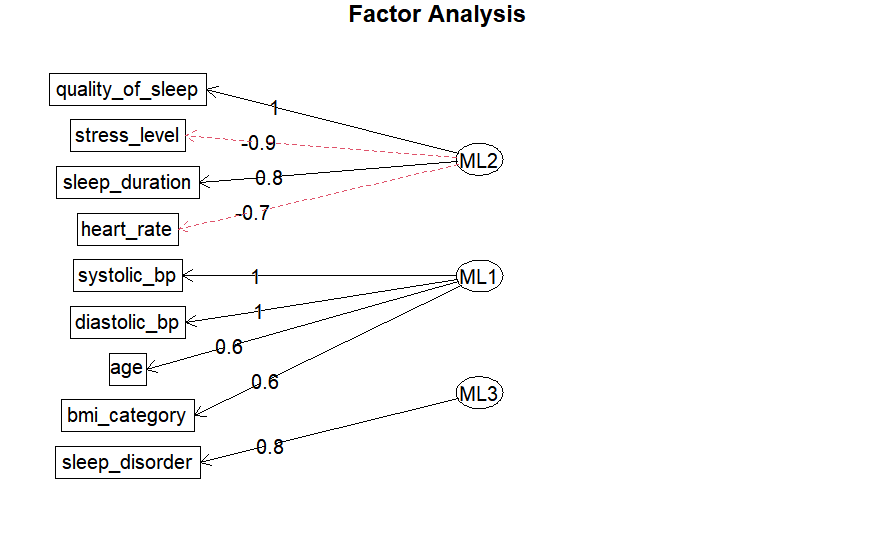
\includegraphics[width=0.7\linewidth]{Images/fa_variax_ml}
			\label{fig:favariaxpa}
		\end{figure}
		
		Based on the factor loadings provided in the table, the following improvements and factor names could be suggested: 
		
		\begin{enumerate}
			
			\item \textbf{Factor Loadings}
			\begin{itemize}
				\item Factor 1 shows strong positive correlations with Systolic Blood Pressure (0.97) and Diastolic Blood Pressure (0.95), indicating that it represents aspects related to blood pressure. Moreover, a moderate positive correlation with Age (0.65) suggests that older individuals tend to have higher blood pressure.
				
				\item Factor 2 exhibits a strong positive correlation with Quality of Sleep (0.97) and a strong negative correlation with Stress Level (-0.93), suggesting that higher levels of stress are associated with lower quality of sleep. Additionally, positive correlations with Sleep Duration (0.85) and Age (0.51) imply that older individuals with longer sleep durations experience higher quality of sleep. The negative correlation with Heart Rate (-0.69) may indicate that lower heart rates are associated with better sleep quality.
				
				\item Factor 3 is positively correlated with BMI category (0.72), indicating that it represents aspects related to body composition. Conversely, it shows a negative correlation with Sleep Disorder (-0.47), suggesting that lower scores on this factor are associated with fewer sleep disorders.
			\end{itemize}
			
			\item \textbf{Communalities}
			
			Another assessment of how well this model performs can be obtained from the communalities. The model performs particularly well in explaining the variation in Quality of Sleep and Systolic Blood Pressure, while also showing relatively strong performance for variables such as Diastolic Blood Pressure, Stress Level, Sleep Duration, Age, Sleep Disorder, and BMI Category. However, the model performs less effectively for Heart Rate, explaining half of the variation.
			
			\item \textbf{Total communality value}
			
			The sum of all communality values is the total communality value = $ 7.261763$. 
			
			\item \textbf{The proportion of total variation explained by the three factors} 
			\begin{center}
				$\frac{7.261763}{9} = 0.8068625$
			\end{center}
			Therefore, 80.69\% proportion of the total variation explained by the three factors.
			
			\item \textbf{Uniqueness}
			
			The uniqueness of a variable represents the variance that is unique to that variable and not shared with other variables. According to this analysis, the uniqueness of Heart Rate is 0.48, it means that 48\% of the variance in Heart Rate is not shared with other variables in the factor model. Conversely, Quality of Sleep and Systolic BP indicate that only 0.4\% of their variance is not accounted for by other variables. It is important to note that, variables with lower uniqueness values are more important in explaining the common variance captured by the factors.
			
		\end{enumerate}
		
		\newpage
		\subsection{Confirmatory Factor Analysis (CFA)}
		CFA is used to assess the overall measurement of a concept when there are
		multiple items available to measure it. 
		
		\begin{tcolorbox}[colback=white,colframe=black]
			\begin{verbatim}
				Test statistic                               314.838
				Degrees of freedom                                23
				P-value (Chi-square)                           0.000
				
				User Model versus Baseline Model:
				
				Comparative Fit Index (CFI)                    0.922
				Tucker-Lewis Index (TLI)                       0.877
				
				Root Mean Square Error of Approximation:
				
				RMSEA                                          0.184
				90 Percent confidence interval - lower         0.166
				90 Percent confidence interval - upper         0.203
				P-value H_0: RMSEA <= 0.050                    0.000
				P-value H_0: RMSEA >= 0.080                    1.000
				
				Standardized Root Mean Square Residual:
				
				SRMR                                           0.071
				
				R^2 Values
				age          quality_of_sleep     stress_level   sleep_duration 	heart_rate      
				0.675               NA            0.807            0.779	          0.435             
				systolic_bp     diastolic_bp     bmi_category 	sleep_disorder 
				0.992            0.954            0.796            0.526 
				
			\end{verbatim}
		\end{tcolorbox}

			\subsubsection{Overall Model Level Fit}
		
			Multiple methods of estimation have been developed for SEM models generally
			and CFA models specifically.
		
			\begin{enumerate}
				\item \textbf{Model Test:} 
				
				The chi-square test assesses the goodness of fit of the model. A lower p-value (close to 0) suggests that the model significantly deviates from the expected values, indicating a potential lack of fit. In this case, with a p-value of 0.000, the model significantly deviates from the expected values.
				
				\item \textbf{Root Mean Square Error of Approximation (RMSEA):}
				
				The root mean square error of approximation is a parsimonyadjusted fit index, meaning that it favors simplicity in models. Lower RMSEA values indicate better fit, with values below 0.05 typically considered good. The provided RMSEA of 0.184 suggests a moderate fit. 
				\newpage
				\item \textbf{Comparative Fit Index (CFI) and Tucker-Lewis Index (TLI):}
				
				These indices assess the model fit by comparing it to a baseline model. Values closer to 1 indicate better fit. Both CFI and TLI values are closer to 1, suggesting a reasonable fit of the model.
				
				\item \textbf{Standardized Root Mean Square Residual (SRMR):}
				
				SRMR measures s the square root
				of the standardized difference between the sample covariances and the covariances predicted by the model. Lower values indicate better fit. The provided SRMR of 0.071 suggests a reasonably good fit.
			\end{enumerate}
		
		Overall, the model appears to have a reasonable fit to the data, although it may not be perfect. Further adjustments or evaluations might be necessary depending on the specific goals of the analysis.
		
		\subsubsection{Equation Level Fit}
			
		The equation-level fit of the model was assessed using R$^2$ values for each observed variable. The model demonstrated strong predictive power for variables such as stress level, sleep duration, systolic and diastolic blood pressure, and BMI category, with R$^2$ values ranging from approximately 79.6\% to nearly 99.2\%. Variables like age and sleep disorder also exhibited moderate to high levels of explained variance (approximately 67.5\% and 52.6\% respectively). Notably, heart rate showed comparatively lower explained variance at around 43.5\%. These results suggest that the model provides a generally good fit for predicting the observed variables.
		
		\subsubsection{Parameter Level Fit}
		
			Factor loadings indicate the strength and direction of the relationship between latent factors and observed variables.
		
			\begin{table}[h]
				\centering
				\resizebox{10cm}{!}{%
					\begin{tabular}{c|ccc|c|}
						\cline{2-5}
						& \multicolumn{3}{c|}{\textbf{$\lambda$}}                                                & \textbf{$\theta$} \\ \cline{2-5} 
						\textbf{}                              & \multicolumn{1}{c|}{\textbf{Factor 1}} & \multicolumn{1}{c|}{\textbf{Factor 2}} & \textbf{Factor 3} & \textbf{Error}                 \\ \hline
						\multicolumn{1}{|c|}{Age}              & \multicolumn{1}{c|}{0.555}             & \multicolumn{1}{c|}{0.676}             & 0.000             & 0.325                          \\ \hline
						\multicolumn{1}{|c|}{Sleep Duration}   & \multicolumn{1}{c|}{1.000}             & \multicolumn{1}{c|}{0.000}             & 0.000             & -0.001                         \\ \hline
						\multicolumn{1}{|c|}{Quality of Sleep} & \multicolumn{1}{c|}{-0.898}            & \multicolumn{1}{c|}{0.000}             & 0.000             & 0.193                          \\ \hline
						\multicolumn{1}{|c|}{Stress Level}     & \multicolumn{1}{c|}{0.883}             & \multicolumn{1}{c|}{0.000}             & 0.000             & 0.221                          \\ \hline
						\multicolumn{1}{|c|}{BMI Category}     & \multicolumn{1}{c|}{-0.659}            & \multicolumn{1}{c|}{0.000}             & 0.000             & 0.565                          \\ \hline
						\multicolumn{1}{|c|}{Systolic BP}      & \multicolumn{1}{c|}{0.000}             & \multicolumn{1}{c|}{0.996}             & 0.000             & 0.008                          \\ \hline
						\multicolumn{1}{|c|}{Diastolic BP}     & \multicolumn{1}{c|}{0.000}             & \multicolumn{1}{c|}{0.977}             & 0.000             & 0.046                          \\ \hline
						\multicolumn{1}{|c|}{Heart Rate}       & \multicolumn{1}{c|}{0.000}             & \multicolumn{1}{c|}{0.000}             & 0.892             & 0.204                          \\ \hline
						\multicolumn{1}{|c|}{Sleep Disorder}   & \multicolumn{1}{c|}{0.000}             & \multicolumn{1}{c|}{0.000}             & 0.725             & 0.474                          \\ \hline
					\end{tabular}%
				}
				%\caption{}
				\label{tab:cfa_factor}
			\end{table} 
		
		In Factor 1, variables like age, sleep duration, and systolic blood pressure have relatively high loadings, suggesting a strong association with the latent factor represented by Factor 1. Conversely, variables like stress level and heart rate show negative loadings, indicating an inverse relationship with Factor 1.
		
		Factor 2 primarily captures variables related to blood pressure (systolic and diastolic), with high loadings on these variables and relatively low loadings on others.
		
		Factor 3 is predominantly associated with BMI category and sleep disorder, with high loadings on these variables and negligible loadings on others.
		
		\begin{tcolorbox}[colback=white,colframe=black]
			\begin{verbatim}				
				$psi
				factr1 factr2 factr3
				factor1  1.000              
				factor2 -0.120  1.000       
				factor3 -0.361  0.795  1.000
			\end{verbatim}
		\end{tcolorbox}
		
		Theta and Psi matrices represent the relationships between factors and error terms. These values indicate the strength of association and covariance between latent factors and any unexplained variance in the observed variables.
		
		Overall, the factor loadings suggest that the model adequately captures the relationships between latent factors and observed variables, providing insights into the underlying structure of the data and informing potential model refinement. Non-significant loadings, such as those for certain variables on Factor 3, may indicate areas for model improvement, possibly through the inclusion of additional variables or modification of the structural model.
		
		\section{Conclusion}
		In conclusion, the Explanatory Factor Analysis (EFA) and Confirmatory Factor Analysis (CFA) conducted on the "Sleep Health and Lifestyle" dataset have revealed three distinct factors that explains various facts of sleep health and overall well-being. Factor 1, identified as the Cardiovascular Health Factor, contains variables related to blood pressure and age, highlighting the critical role of cardiovascular health in sleep quality. Factor 2, named the Sleep Wellness Factor, includes variables associated with sleep duration, quality, and stress levels, highlighting relationship between sleep patterns and psychological well-being. Finally, Factor 3, the Body-Mind Balance Factor, reflects variables related to body composition and sleep disorders, emphasizing the inter connection of physical and mental health with sleep quality.
		
		These factors offer valuable insights for healthcare professionals, researchers, and policymakers looking to create specific measures to improve sleep quality and promote overall well-being. Understanding the different dimensions of sleep health and lifestyle factors allows for the development of customized solutions to address the specific needs and challenges that individuals in various populations face. Furthermore, the discovery of these factors emphasizes the importance of taking a variety of perspectives when it comes to sleep health management.
		
		\newpage
		\section{References}
		\begin{enumerate}
			\item CitedDemir, Ergul. “RPubs - Intro to EFA and CFA in R.” Rpubs.com, 2022, \url{rpubs.com/isbell_daniel/efa_cfa_intro}. Accessed 7 Apr. 2024.
			
			\item Example of Factor Analysis Method Section Reporting. Huang, Gaoping. “Exploratory Factor Analysis -- Notes and R Code · Gaoping Huang’s Blog.” Gaopinghuang0.Github.io, 9 Feb. 2018, \url{gaopinghuang0.github.io/2018/02/09/exploratory-factor-analysis-notes-and-R-code}. Accessed 23 Nov. 2022.
			
			\item Isbell, Dan. “RPubs - MyClassNotes\_EFA\_CFA.” Rpubs.com, 17 Apr. 2021, \url{rpubs.com/Symrna/EFA_CFA}.
			
			\item Murphy, Phil. “RPubs - Exploratory Factor Analysis in R.” Rpubs.com, 21 Apr. 2021, \url{rpubs.com/pjmurphy/758265}.
			
			\item THARMALINGAM, LAKSIKA. “Sleep Health and Lifestyle Dataset.” \url{www.kaggle.com}, Oct. 2023, \url{https://www.kaggle.com/datasets/uom190346a/sleep-health-and-lifestyle-dataset}.
		\end{enumerate}
		

		\section{Appendices}
		
			\begin{figure}[h]
				\includegraphics[width=12cm]{Images/"Screenshot (14)"}
				\label{fig:r_code1}
			\end{figure}
			
			\begin{figure}[b]
				\includegraphics[width=10cm]{Images/"Screenshot (15)"}
				\label{fig:r_code1}
			\end{figure}
			
			\begin{figure}[!]
				\includegraphics[width=10cm]{Images/"Screenshot (16)"}
				\label{fig:r_code1}
			\end{figure}
			

			\begin{figure}[!]
				\includegraphics[width=10cm]{Images/"Screenshot (17)"}
				\label{fig:r_code1}
			\end{figure}
			
			\begin{figure}[!]
				\includegraphics[width=10cm]{Images/"Screenshot (18)"}
				\label{fig:r_code1}
			\end{figure}
			
			\begin{figure}[!]
				\includegraphics[width=10cm]{Images/"Screenshot (19)"}
				\label{fig:r_code1}
			\end{figure}
			
			\begin{figure}[!]
				\includegraphics[width=10cm]{Images/"Screenshot (20)"}
				\label{fig:r_code1}
			\end{figure}
		
		
		
\end{document}
